%
% Authors
% Denis Augsburger
% Pierro Steinger
% Thomas Wilde
% Nicolas Mauchle
% 
%
% Version 0.1
%
\documentclass[12pt,a4paper,german]{article}
%
\author{Denis Augsburger, Pierro Steinger, Thomas Wilde, Nicolas Mauchle, }
%
\usepackage[left=2.5cm,right=2.5cm,bottom=2.5cm,includeheadfoot]{geometry}
\usepackage[pdftex]{graphicx}
\usepackage{babel}
\usepackage[utf8]{inputenc}
\usepackage{fancyhdr}
\usepackage{lastpage}
%
% Graue Farbe
\usepackage{blindtext} 
\usepackage{framed} 
\usepackage{xcolor} 
\colorlet{shadecolor}{gray!25} 
 \usepackage{color}
\input{utils/colors}

\usepackage{hyperref}
\hypersetup{
    pdfborder = {0 0 0}
}
 \usepackage{mathpazo}
% \linespread{1.5}
%Damit man label setzten kann wo man will
\usepackage[all]{hypcap}
%

\usepackage[stable]{footmisc}
% KOPF UND FUSS ZEILEN
\pagestyle{fancy}
%
\fancyhf[R]{}
\fancyhf[L]{\leftmark}
%
% suppress page number in bottom center:
\cfoot{}
%
\fancyfoot[L]{}
\fancyfoot[R]{Seite \thepage \  von  \pageref{LastPage}}
%
%Linie unten
\renewcommand{\footrulewidth}{0.5pt}
%
\newcommand{\HRule}{\rule{\linewidth}{0.5mm}}
%\title{Über den Prozess der Zivilisation}
\begin{document}
%\maketitle
\begin{titlepage}
\begin{center}
\textsc{\LARGE Fachhochschule Nordwestschweiz}\\[1.5cm]
% Title
\HRule \\[0.4cm]
{ \huge \bfseries Portfolio}\\[0.4cm]
\HRule \\[1.5cm]
% Author and supervisor
\begin{minipage}{1.2\textwidth}
\begin{flushleft} \large
\emph{Autor:}\\
Lea Knöll
\newline
\newline
\emph{Dozent:} \\
René Fankhauser
\newline
\newline
\emph{Klasse:} \\
3. Semester\\
%\end{flushright}
\end{flushleft}
\end{minipage}
\vfill
% Bottom of the page
{\large \today}
\end{center}
\end{titlepage}

\newpage
\tableofcontents


\section{Einleitung}
Für die Firma Nutz AG soll eine neue Applikation entwickelt werden, um die Vermietung und Wartung der Fahrzeuge zielgerichteter anzubieten.\\
Zurzeit hat die Firma ca. 200 verschiedene Nutzfahrzeuge. Ihre Kundendatenbank umfasst über 3000 Privat- sowie auch Geschäftskunden.\\
Durch die verschiedenen Standorte, kommt es immer wieder zu unnötigen Fahrzeugverschiebungen. Auch die Wartung der Fahrzeuge wir momentan mit einer Excelliste rapportiert.\\[2ex]
%
Dies soll durch die neue Webapplikation verbessert und vereinfacht werden.\\
Auf den nächsten Seiten werden die Stakeholder nach ihrer Wichtigkeit identifiziert, in Interessengruppen einteilen.\\
Danach werden wir Probleme sowie Widerstände aufzeigen, die im Verlauf des Projektes auftretten könnten.\\
Um an die richtigen Informationen zu gelnagen, zeigen wir für jede Interessegruppe unsere Idee für die \textit{Erhebung der Informtionen} auf.\\
Durch das Kontextdiagramm veranschulichen wir den ganzen Arbeitsprozess\\
Zum Schluss definieren wir noch unsere Ziele, die wir in diesem Projekt erreichen möchten.
% LaTeX n00bs indent stuff
\newpage

% Aufgabe 1) Interessengruppen identifizieren & analysieren
% Beschreiben der Interessengruppe
\section{Interessengruppen}
%
Wir haben folgende Interessengruppen gefunden.
\begin{center}
  \begin{figure}[ht]
    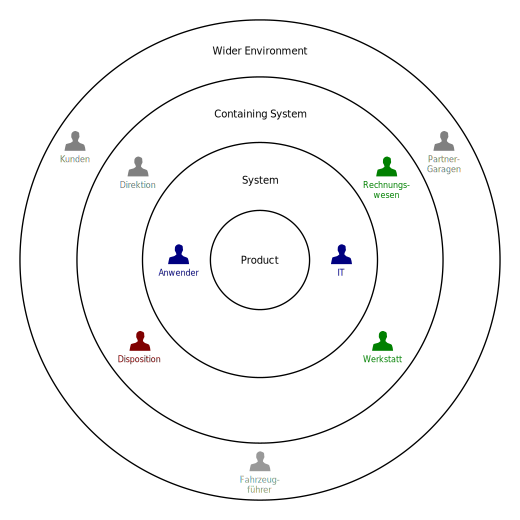
\includegraphics{aufgabe1/graphics/onion.pdf}
    \caption{Onion-Diagramm der Nutz AG Steakholders}
    \label{fig:awesome_image}
  \end{figure}
\end{center}
%
\textbf{Anwender}\\
Die Anwender sind für die Verwaltung des Fahrzeugparks zuständig. Es handelt sich meist um Angestellte mit einem kaufmännischen Hintergrund.Sie möchten mit dem System bestehende Abläufe möglichst einfach ausführen. 
\\[6ex]
%
\textbf{IT}\\
Die IT besteht aus 3 Mitarbeitern im Support. Komplexere Aufgaben werden mit externen Partnern realisiert. Ein AS400-System ist im Einsatz und der Wartungsvertrag läuft in 14 Monaten aus. Dies ist der Endtermin aus Sicht der IT. Der IT-Verantwortliche hat klare Vorstellungen an das neue System, welche teilweise ausserhalb des Einsatzgebietes liegen. Die Software soll umfangreich und trotzdem einfach nutzbar sein. Die Wartungsarbeiten an Serversystemen soll für den Support minimiert werden.
\\[2ex]
\textbf{Rechnungwesen}\\
Das Rechnungswesen möchte die Kosten um 20\% mit dem Projekt senken. Das Berichtswesen soll ausgebaut werden. Die Zahlungsmoral soll verbessert werden, beispielsweise durch eine "realtime" Debitorenbuchhaltung. Ebenfalls soll eine Auswertung der Debitoren nach Kunden, Kundengruppen, Fahrzeugkategorien möglich sein. Diese Auswertung dient den Führungskräften zur Kommunikation gegen Innen und Aussen. Ziel für das Rechnungswesen ist es den Gewinn zu optimieren.
\\[2ex]
\textbf{Disposition}\\
Die Disposition ist verantwortlich, dass sich die Fahrzeuge zum richtigen Zeitpunkt am richtigen Ort befinden. Die interne Organisation ist den Beteiligten klar. Bestehende Arbeitsabläufe sollen möglichst nicht verändert werden, da diese bereits mehrmals optimiert wurden.
\\[2ex]
\textbf{Direktion}\\
Der Direktor hat noch kein konkretes Budget erstellt. Die Obergrenze für das Projekt befindet sich zwischen 600'000 - 800'000 CHF. Er möchte keine Unruhe mit dem Projekt stiften, da er bald in Pension geht.
\\[2ex]
\textbf{Weitere Stakeholder}\\
Die Fahrzeuge dürfen nur im Inland eingesetzt werden. Wir vermuten wegen Versicherungsbedingungen und fehlendem Pannendienst. \\
Die Garagen müssen im Vorfeld über den Einsatz des Mietfahrzeugs in Ihrer Region informiert werden. Diese möchten für entsprechende Pannen im Vorfeld disponieren. \\
Die Kunden erwarten einen reibungslosen Ablauf bei der Miete der Fahrzeuge. Umständliche Formalitäten und lange Wartezeiten sollten möglichst vermieden werden.
\newpage
\section{Mögliche Widerstände}
  \subsection{Dispositionsabteilung}
  Laut dem Abteilungschef läuft der bestehende Prozess einwandfrei. Es besteht eine Tendenz gegen die Erarbeitung der neuen Plattform.
  Der Firmendirektor meinte, es hätte mehrmals Diskussionen darüber gegeben.\\
  %
  Der Abteilungschef sollte im Informationsfluss mit einbezogen werden. Ziel ist, ihn dennoch von den Vorteilen des neuen Systems zu überzeugen.
  %
  \subsection{Low-Profile}
  Die Direktion wünscht sich eine nicht-zu-invasive Entwicklungsphase, was das Requirement Engineering etwas schwieriger macht.\\
  %
  Mit guter Vorbereitung und wenigen, jedoch gezielten Terminen mit wenigen Personen könnte der "Aufdringlichkeitsfaktor" reduziert werden. 
  %
  \subsection{Projektleitung}
  Der IT-Chef als interner Projektleiter scheint nicht sehr gut qualifiziert zu sein. Dazu steht er unter viel Stress.
\newpage
\section{Probleme und fehlende Informationen}


\end{document}
